\documentclass{beamer}
\usepackage[utf8]{inputenc}

\usetheme{Madrid}
\usecolortheme{default}
\usepackage{amsmath,amssymb,amsfonts,amsthm}
\usepackage{txfonts}
\usepackage{tkz-euclide}
\usepackage{listings}
\usepackage{adjustbox}
\usepackage{array}
\usepackage{tabularx}
\usepackage{gvv}
\usepackage{lmodern}
\usepackage{circuitikz}
\usepackage{tikz}
\usepackage{graphicx}

\setbeamertemplate{page number in head/foot}[totalframenumber]

\usepackage{tcolorbox}
\tcbuselibrary{minted,breakable,xparse,skins}



\definecolor{bg}{gray}{0.95}
\DeclareTCBListing{mintedbox}{O{}m!O{}}{%
	breakable=true,
	listing engine=minted,
	listing only,
	minted language=#2,
	minted style=default,
	minted options={%
		linenos,
		gobble=0,
		breaklines=true,
		breakafter=,,
		fontsize=\small,
		numbersep=8pt,
		#1},
	boxsep=0pt,
	left skip=0pt,
	right skip=0pt,
	left=25pt,
	right=0pt,
	top=3pt,
	bottom=3pt,
	arc=5pt,
	leftrule=0pt,
	rightrule=0pt,
	bottomrule=2pt,
	toprule=2pt,
	colback=bg,
	colframe=orange!70,
	enhanced,
	overlay={%
		\begin{tcbclipinterior}
			\fill[orange!20!white] (frame.south west) rectangle ([xshift=20pt]frame.north west);
	\end{tcbclipinterior}},
	#3,
}
\lstset{
	language=C,
	basicstyle=\ttfamily\small,
	keywordstyle=\color{blue},
	stringstyle=\color{orange},
	commentstyle=\color{green!60!black},
	numbers=left,
	numberstyle=\tiny\color{gray},
	breaklines=true,
	showstringspaces=false,
}
\begin{document}

\title 
{2.4.37}
\date{6 September,2025}

\author 
{Naman Kumar-EE25BTECH11041}
\graphicspath{./figs}


\frame{\titlepage}
\begin{frame}{Question}
Find a vector of magnitude 6, which is perpendicular to both the vectors $2\hat{\imath} - \hat{\jmath} + 2\hat{k}$ and $4\hat{\imath} - \hat{\jmath} + 3\hat{k}$\\
\end{frame}
\begin{frame}{Equation Used}
Inner Product,
\begin{align}
    \vec{A} \cdot \vec{B}
\end{align}
Also Rank of matrix
\end{frame}
\begin{frame}{Solution}
Given Vectors
\begin{align}
    \Vec{A}=\begin{pmatrix} 2\\-1\\2 \end{pmatrix}, \Vec{B}=\begin{pmatrix} 4\\-1\\3 \end{pmatrix}
\end{align}
Let required vector be,
\begin{align}
    \vec{C}=\begin{pmatrix} x\\y\\z \end{pmatrix}
\end{align}
\end{frame}
\begin{frame}{Solution}
Using Inner Product,
\begin{align}
    \vec{C}^T \cdot\vec{A}=0\text{ and }\vec{C}^T \cdot\vec{B}=0\\
    \vec{C}^T \cdot\vec{A}=2x-y+2z=0 \label{1} \\
    \vec{C}^T \cdot\vec{B}=4x-y+3z=0 \label{2}
\end{align}
Using Row Transformations to Get Row Reduced echelon Form
\begin{align}
    \vec{A}=\begin{pmatrix} 2&-1&2\\4&-1&3 \end{pmatrix} \xrightarrow[]{R_2 \rightarrow R_2-2R_1}\begin{pmatrix} 2&-1&2\\0&1&-1 \end{pmatrix}\\
    \xrightarrow[]{R_1 \rightarrow \frac{1}{2}R_1}\begin{pmatrix} 1&\frac{-1}{2}&1\\0&1&-1 \end{pmatrix}\\
    \xrightarrow[]{R_1 \rightarrow R_1+\frac{1}{2}R_2}\begin{pmatrix} 1&0&\frac{1}{2}\\0&1&-1 \end{pmatrix}
\end{align}
\end{frame}
\begin{frame}{Solution}
\begin{align}
\vec{A}=(\vec{I}\vec{X}), \text{\textbf{I} is identity matrix}
\end{align}
And, $\vec{X}$ is
\begin{align}
    \begin{pmatrix}\frac{1}{2}\\-1\end{pmatrix}
\end{align}
Since rank of matrix is 2($\leq 3$), their are infinite many solutions $R^3\rightarrow R^2$\\
From the Row Reduced Echelon form(RREF),we can write the new system of equation:
\begin{align}
    x+\frac{1}{2}z=0 \label{3} \\
    y-z=0 \label{4}
\end{align}
\end{frame}
\begin{frame}{Solution}
Therefore vector $\vec{C}$ using equations $\eqref{3}$ and $\eqref{4}$ is
\begin{align}
    \vec{C}=\begin{pmatrix}x\\-2x\\-2x\end{pmatrix}=x\begin{pmatrix}1\\-2\\-2\end{pmatrix}
\end{align}
Now getting vector with magnitude 6
\begin{align}
    \lVert C\rVert =6\\
    \lVert x\rVert \sqrt{(1)^2+(-2)^2+(-2)^2}=6\\
    \lVert x\rVert \sqrt{1+4+4}=6\\
    \lVert x\rVert \sqrt{9}=6\\
    \lVert x\rVert =2
\end{align}
\end{frame}
\begin{frame}{Solution}
Therefore final vectors are
\begin{align}
    C_1=\begin{pmatrix} -2\\4\\4 \end{pmatrix},
    C_2=\begin{pmatrix} 2\\-4\\-4 \end{pmatrix}
\end{align}
\end{frame}
\begin{frame}{Figure}
    \begin{figure}
        \centering
        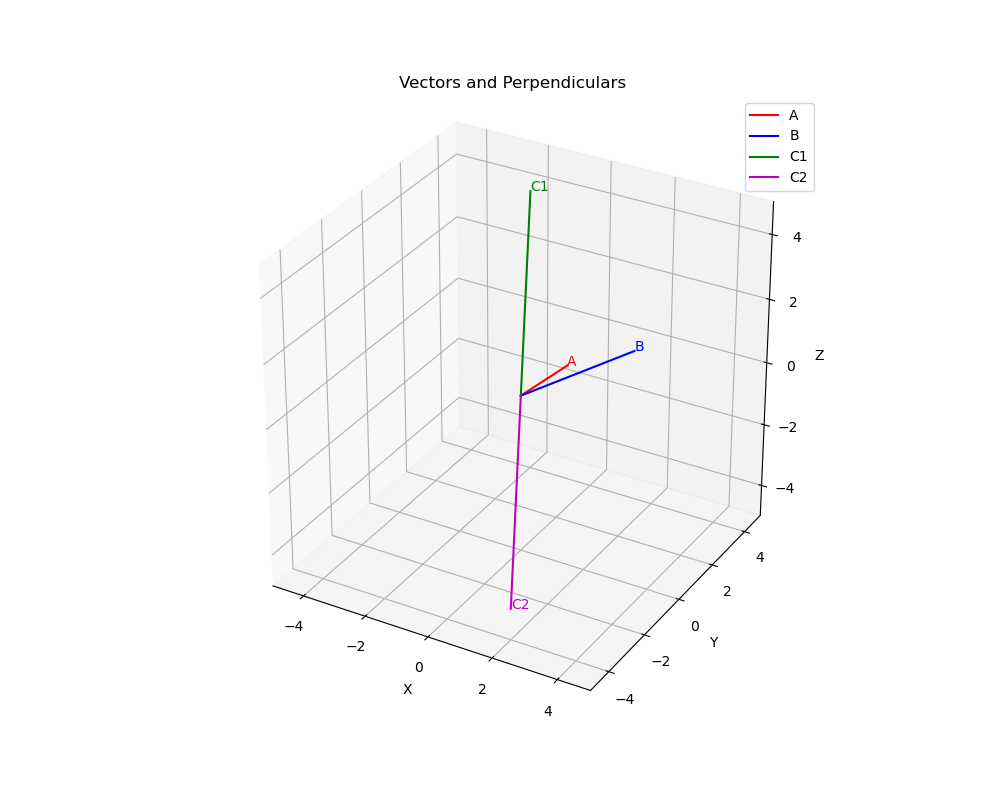
\includegraphics[width=\columnwidth]{figs/vector_plot.png}
        \caption{Caption}
        \label{fig:placeholder}
    \end{figure}
\end{frame}

\begin{frame}[fragile]
\frametitle{C code}
\begin{lstlisting}
#include <math.h>

// Compute cross product of two 3D vectors
void cross_product(double *a, double *b, double *result) {
    result[0] = a[1]*b[2] - a[2]*b[1];
    result[1] = a[2]*b[0] - a[0]*b[2];
    result[2] = a[0]*b[1] - a[1]*b[0];
}

// Compute magnitude of a 3D vector
double magnitude(double *v) {
    return sqrt(v[0]*v[0] + v[1]*v[1] + v[2]*v[2]);
}
\end{lstlisting}
\end{frame}
\begin{frame}[fragile]
\frametitle{C code}
\begin{lstlisting}
// Given a, b, and desired magnitude, compute two perpendicular vectors of that magnitude
// Output: v1[3], v2[3]
void perpendicular_vectors(double *a, double *b, double mag, double *v1, double *v2) {
    double c[3];
    cross_product(a, b, c);

    double norm_c = magnitude(c);

    if (norm_c == 0.0) { 
        // Parallel vectors → cross product is zero
        v1[0] = v1[1] = v1[2] = 0.0;
        v2[0] = v2[1] = v2[2] = 0.0;
        return;
    }
\end{lstlisting}
\end{frame}
\begin{frame}[fragile]
\frametitle{C code}
\begin{lstlisting}
    // Normalize c
    double c_hat[3];
    c_hat[0] = c[0] / norm_c;
    c_hat[1] = c[1] / norm_c;
    c_hat[2] = c[2] / norm_c;

    // Scale to desired magnitude
    v1[0] = mag * c_hat[0];
    v1[1] = mag * c_hat[1];
    v1[2] = mag * c_hat[2];

    v2[0] = -v1[0];
    v2[1] = -v1[1];
    v2[2] = -v1[2];
}
\end{lstlisting}
\end{frame}

\begin{frame}[fragile]
\frametitle{Python Code through SO file}
\begin{lstlisting}
import ctypes
import numpy as np
import matplotlib.pyplot as plt

# Load C shared object
lib = ctypes.CDLL("./main.so")

# Define argument and return types
lib.perpendicular_vectors.argtypes = [
    ctypes.POINTER(ctypes.c_double), # a
    ctypes.POINTER(ctypes.c_double), # b
    ctypes.c_double,                 # magnitude
    ctypes.POINTER(ctypes.c_double), # v1
    ctypes.POINTER(ctypes.c_double)  # v2
]
lib.perpendicular_vectors.restype = None
\end{lstlisting}
\end{frame}

\begin{frame}[fragile]
\frametitle{Python Code through SO file}
\begin{lstlisting}
# Given vectors
a = np.array([2.0, -1.0, 2.0], dtype=np.double)
b = np.array([4.0, -1.0, 3.0], dtype=np.double)
magnitude = 6.0

# Prepare outputs
v1 = np.zeros(3, dtype=np.double)
v2 = np.zeros(3, dtype=np.double)

# Call C function
lib.perpendicular_vectors(
    a.ctypes.data_as(ctypes.POINTER(ctypes.c_double)),
    b.ctypes.data_as(ctypes.POINTER(ctypes.c_double)),
    magnitude,
    v1.ctypes.data_as(ctypes.POINTER(ctypes.c_double)),
    v2.ctypes.data_as(ctypes.POINTER(ctypes.c_double))
)
\end{lstlisting}
\end{frame}

\begin{frame}[fragile]
\frametitle{Python Code through SO file}
\begin{lstlisting}
print(f"Vector a: {a}")
print(f"Vector b: {b}")
print(f"First perpendicular vector v1 (|v1|={np.linalg.norm(v1):.2f}): {v1}")
print(f"Second perpendicular vector v2 (|v2|={np.linalg.norm(v2):.2f}): {v2}")

# --- Plotting ---
fig = plt.figure(figsize=(10, 8))
ax = fig.add_subplot(111, projection='3d')
origin = [0, 0, 0]

ax.plot([0,a[0]], [0,a[1]], [0,a[2]], color='r', label='A')
ax.plot([0,b[0]], [0,b[1]], [0,b[2]], color='b', label='B')
\end{lstlisting}
\end{frame}

\begin{frame}[fragile]
\frametitle{Python Code through SO file}
\begin{lstlisting}
ax.plot([0,v1[0]], [0,v1[1]], [0,v1[2]], color='g', label='V1')
ax.plot([0,v2[0]], [0,v2[1]], [0,v2[2]], color='m', label='V2')

ax.text(a[0], a[1], a[2], 'A', color='r')
ax.text(b[0], b[1], b[2], 'B', color='b')
ax.text(v1[0], v1[1], v1[2], 'C1', color='g')
ax.text(v2[0], v2[1], v2[2], 'C2', color='m')

max_val = np.max(np.abs(np.vstack((a, b, v1, v2)))) * 1.2
ax.set_xlim([-max_val, max_val])
ax.set_ylim([-max_val, max_val])
ax.set_zlim([-max_val, max_val])
ax.set_xlabel('X')
\end{lstlisting}
\end{frame}

\begin{frame}[fragile]
\frametitle{Python Code through SO file}
\begin{lstlisting}
ax.set_ylabel('Y')
ax.set_zlabel('Z')
ax.set_title('Vectors and Perpendiculars')
ax.legend()
ax.grid(True)
ax.set_box_aspect([1,1,1])

plt.savefig('vector_plot.png')

plt.show()
\end{lstlisting}
\end{frame}

\begin{frame}[fragile]
\frametitle{Direct Python Code}
\begin{lstlisting}
# Inspired by code from GVV Sharma
# September 5, 2024
# released under GNU GPL
# Find two vectors of magnitude 6 perpendicular to two given vectors and plot them.

import numpy as np
import matplotlib.pyplot as plt
from mpl_toolkits.mplot3d import Axes3D

# Given vectors
a = np.array([2, -1, 2])
b = np.array([4, -1, 3])

# To find a vector perpendicular to both a and b, we compute their cross product.
c = np.cross(a, b)
\end{lstlisting}
\end{frame}

\begin{frame}[fragile]
\frametitle{Direct Python Code}
\begin{lstlisting}
print(f"Vector 'a': {a}")
print(f"Vector 'b': {b}")
print(f"Vector perpendicular to a and b (a x b = c): {c}")

# Now, we need a vector of magnitude 6 in the direction of c.
# First, find the unit vector in the direction of c.
# Magnitude of c
norm_c = np.linalg.norm(c)
# Unit vector c_hat
c_hat = c / norm_c

print(f"Magnitude of c: {norm_c:.2f}")
print(f"Unit vector in the direction of c: {c_hat}")
\end{lstlisting}
\end{frame}

\begin{frame}[fragile]
\frametitle{Direct Python Code}
\begin{lstlisting}
# Define the desired magnitude
magnitude = 6

# Calculate the final vector v and its opposite
v1 = magnitude * c_hat
v2 = -v1

print(f"The first required vector 'v1' of magnitude {magnitude} is: {v1}")
print(f"The second required vector 'v2' of magnitude {magnitude} is: {v2}")
print(f"Verification: Magnitude of v1 is {np.linalg.norm(v1):.2f}")
print(f"Verification: Magnitude of v2 is {np.linalg.norm(v2):.2f}")
\end{lstlisting}
\end{frame}

\begin{frame}[fragile]
\frametitle{Direct Python Code}
\begin{lstlisting}

# --- Plotting the vectors ---
fig = plt.figure(figsize=(10, 8))
ax = fig.add_subplot(111, projection='3d')

# Origin point
origin = [0, 0, 0]

# Plotting the vectors as lines from origin
ax.plot([origin[0], a[0]], [origin[1], a[1]], [origin[2], a[2]], color='r', label='A = [2, -1, 2]')
ax.plot([origin[0], b[0]], [origin[1], b[1]], [origin[2], b[2]], color='b', label='B = [4, -1, 3]')
ax.plot([origin[0], v1[0]], [origin[1], v1[1]], [origin[2], v1[2]], color='g', label=f'Result C1 = [{v1[0]:.0f}, {v1[1]:.0f}, {v1[2]:.0f}]')
\end{lstlisting}
\end{frame}

\begin{frame}[fragile]
\frametitle{Direct Python Code}
\begin{lstlisting}
ax.plot([origin[0], v2[0]], [origin[1], v2[1]], [origin[2], v2[2]], color='m', label=f'Result C2 = [{v2[0]:.0f}, {v2[1]:.0f}, {v2[2]:.0f}]')

# Adding text labels at the end of each vector
ax.text(a[0]*1.1, a[1]*1.1, a[2]*1.1, 'A', color='r', fontsize=12)
ax.text(b[0]*1.1, b[1]*1.1, b[2]*1.1, 'B', color='b', fontsize=12)
ax.text(v1[0]*1.1, v1[1]*1.1, v1[2]*1.1, 'C1', color='g', fontsize=12)
ax.text(v2[0]*1.1, v2[1]*1.1, v2[2]*1.1, 'C2', color='m', fontsize=12)

\end{lstlisting}
\end{frame}

\begin{frame}[fragile]
\frametitle{Direct Python Code}
\begin{lstlisting}
# Setting the plot limits to be symmetric and encompass all vectors
max_val = np.max(np.abs(np.vstack((a, b, v1)))) * 1.2
ax.set_xlim([-max_val, max_val])
ax.set_ylim([-max_val, max_val])
ax.set_zlim([-max_val, max_val])

# Adding labels and title
ax.set_xlabel('X axis')
ax.set_ylabel('Y axis')
ax.set_zlabel('Z axis')
ax.set_title('Perpendicular Vector Visualization')
ax.legend()
ax.grid(True)
\end{lstlisting}
\end{frame}

\begin{frame}[fragile]
\frametitle{Direct Python Code}
\begin{lstlisting}
# Change the viewing angle (elevation, azimuth)
ax.view_init(elev=25, azim=-45)

# To make the aspect ratio equal
ax.set_box_aspect([1,1,1]) 

# Save the figure as a PNG file
plt.savefig('vector_plot.png')

# Show the plot
plt.show()


\end{lstlisting}
\end{frame}


\end{document}